\chapter{Data}
\section{Common Crawl}
The raw data used for creating the data set was taken from \emph{CommonCrawl}\footnote{http://commoncrawl.org (Last checked: xx.xx.xxxx)}. CommonCrawl is a non-profit organization which crawls the web and releases the data and meta data with almost no restrictions.
In this master thesis, the crawl data from XXXX is used. The data was further processed: HTML was stripped out and it was splitted into sentences with XXXXXXXXX\footnote{This preprocessing was not done by me; source etc.}. To make the data maintainable, the sentences where imported into an ElasticSearch index. The resulting index is XXXX tb big and contains XXXXX sentences. Of those, 32946247 match \texttt{better OR worse}, 4928112 \texttt{"better than" OR "worse than"}. Given that, I expect the data to contain thousands of comparative sentences.

\section{Crowd Sourcing}
\subsection{Data Selection and Preprocessing}
\label{sec:prestudy-processing}
The test sentences were extracted from the ElasticSearch index build from the CommonCrawl data. Query \ref{lst:es-query-a} was used to retrieve sentences containing the two objects of interest and at least one of the words \emph{better, worse, superior} or \emph{inferior}. Like \cite{Daxenberger2017What-is-the-Ess} show that the appearance of certain words mark a claim, I expect that this query returns more comparative sentences because the additional words (\emph{better, ...}) are commonly used in comparisons. As there are many ways to phrase a comparison, Query \ref{lst:es-query-b} was used to retrieve other sentences containing the objects of interest.

\begin{lstlisting}[label=lst:es-query-a,breaklines=true,postbreak=\mbox{\textcolor{red}{$\hookrightarrow$}\space}]
  {
        "query" : {
            "bool": {
                "must": [
                    {
                        "query_string": {
                            "default_field" : "text",
                            "query" :  "(better OR worse OR superior OR inferior) AND \"<OBJECT_A>\" AND \"<OBJECT_B>\""
                        }
                    }
                ]
            }
        }
    }
\end{lstlisting}

\begin{lstlisting}[label=lst:es-query-b,breaklines=true,postbreak=\mbox{\textcolor{red}{$\hookrightarrow$}\space}]
  {
        "query" : {
            "bool": {
                "must": [
                    {
                        "query_string": {
                            "default_field" : "text",
                            "query" :  "\"<OBJECT_A>\" AND \"<OBJECT_B>\""
                        }
                    }
                ]
            }
        }
    }
\end{lstlisting}

It is expected that query \ref{lst:es-query-b}  will add more non-comparative sentences, only 25\% of the sentences used are from this one.

The retrieved sentences where further filtered and pre-processed. Each sentence must be between 15 and 200 characters long, it must contain each of the two objects exactly once (which makes the feature creation easier) and it is not allowed to have more than seven punctuation characters (to exclude lists and the like). In each sentences which fulfills those criteria, \emph{:[OBJECT\_A]} was appended to the first object appearing in the sentence, likewise \emph{:[OBJECT\_B]} for the latter one (see example \ref{exp:sentence}). This was done to make it easier for the annotators to identify the objects of interest.

\begin{ebox}{Preprocessed sentence}
\label{exp:sentence}
\enquote{The apps for the iphone are generally better than those for android}
\tcblower
\enquote{The apps for the iphone:[OBJECT\_A] are generally better than those for android:[OBJECT\_B]}
\end{ebox}


\subsection{Annotation Guidelines}
The annotators where asked to assign one of the four following classes to each sentence (the full guidelines used can be found in the appendix).

\paragraph{BETTER} This class should be used if the sentence indicates that object A (the first object of interest mentioned in the sentence) is better in any way than object B.

\paragraph{WORSE} Same as \emph{BETTER}, but the sentence must indicate that object A is worse than object B.
% A side-effect is very likely to be an increased status for OBJECT_A, probably gradually approaching the status of OBJECT_B, because for many people money really does talk.
\paragraph{UNCLEAR} If the sentence contains an argument, but it is not between A and B, this class should be used.

%Proves Superior to OBJECT_A, OBJECT_B, Perl and Other Dynamic Programming Languages

% OBJECT_A, OBJECT_B, WordPress, and the old standard OpenOffice (in a freshly minted version 4) are better and stronger than ever.

%It's better than any OBJECT_A or OBJECT_B phone I've tested thus far.

%If you shy away from saltimbocca because you don't eat veal, then do yourself a favor and try this twist on the classic Roman dish, which uses OBJECT_A in place of OBJECT_B.
\paragraph{NO\_COMP} All other sentences fall into this category.
%Owning an OBJECT_A or OBJECT_B smartphone just got even better with Pebble , the first watch designed for the 21st century.
%Two recent studies about OBJECT_A and OBJECT_B behavior have reignited the age-old debate about which pet is better.
\newline

In a first version of the guidelines, arguments where the objects (see \ref{exp:unclear}) are not clear should fall into \emph{NO\_COMP} instead of \emph{UNCLEAR}. The intention was that those sentences will decrease the performance of machine learning models as the might be harder to identifiy the compared objects of this sentence correctly.

\begin{ebox}{Argument with unclear objects}
\label{exp:unclear}
Task: Identify comparisons between \emph{Linux} and \emph{Windows}.\\
\enquote{It has a better performance than Linux and Windows}
\end{ebox}

However, this restriction was dropped as the loss of information and the potential confusion of the might be more harmful than the missing object.


\label{sec:annotation-guidelines}
\subsection{Prestudy}
Previous to the crowd sourcing campaign, a pre-study was conducted to assess the quality of the annotation guidelines. For this, 100 sentences for each of the ten object pairs (see table \ref{tbl:prestudy-objects}) where obtained as described in section \ref{sec:prestudy-processing}.

\begin{table}[h]
\centering
\caption{Objects of the Annotation Prestudy}
\label{tbl:prestudy-objects}
\begin{tabular}{@{}lll@{}}
\toprule
First Object & Second Object                                      \\ \midrule
Ruby         & Python                                     \\
Android      & iPhone          \\
Cat          & Dog                                            \\ 
Car & Bicycle  \\
Summer & Winter  \\
BMW & Mercedes  \\
Wine & Beer  \\
USA & Europe  \\
Football             &          Baseball       \\       \midrule                                  
\end{tabular}
\end{table}

The pairs where chosen to obtain a wide range of different objects, which will lead to different comparisons. Some sentences contain programming- and computer specific terms, so a need for this knowledge was expressed.

A first experiment was started with 110 sentences.. Ten sentences where test sentences where the correct answer was known. This is used to filter out people who did not read the annotation guidelines. In this experiment, the original names of the object where removed from the sentence entirely and the first version of the annotation guidelines where used. The results showed that the amount of test sentences was to small, and that the phrasing of the four classes was not optimal.\newline

This (and the reasons mentioned above) lead to the updated annotation guidelines and better class descriptions. In the second experiment, 251 sentences (51 test sentences) where used. Furthermore, the sentences looked as described in example \ref{exp:sentence}, also the objects where highlighted by different colors (purple for object A, green for object B). Each sentence was annotated by three annotators. The resulting class distribution is shown in figure \ref{pre:dist}

\begin{figure}[h]
\centering
\caption{Class Distribution in the prestudy}
\label{pre:dist}
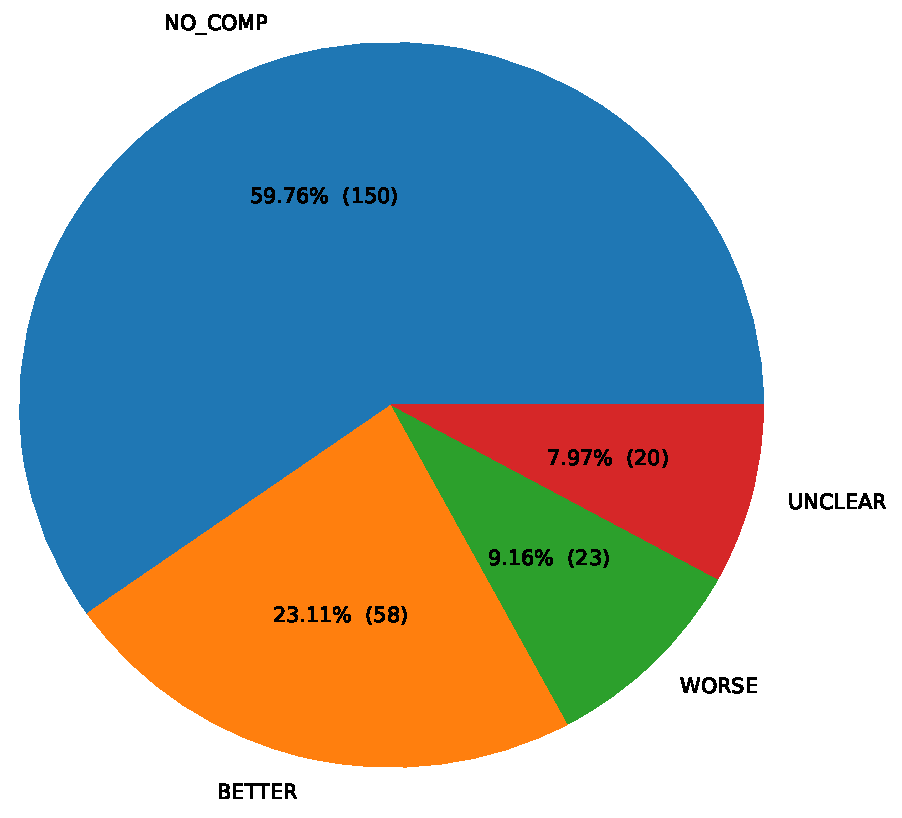
\includegraphics[scale=0.6]{images/prestudy/label_distribution.pdf}
\end{figure}

This distribution is similar to the distribution of classes from all 1000 sentences (labeled by me) \ldots

As a measure for quality, CrowdFlower calculates the \emph{confidence} for each label. For each annotator, CrowdFlower has a trust level between 0 and 1. Every time an annotator annotates a sentence with a class, the confidence of the class increases by $0.33 \times trust$ (0.33 because each sentence is annotated by three annotators). In this way, a confidence of one is achieved if each of the three annotators has a trust level of one and each one uses the same class. (CHECK)

The average trust was XXX with a standard derivation of YYY. Lowest trust was ZZZ.


As presented in figure \ref{pre:dist}, a majority (151) of the labellings has a confidence greater or equal to 0.9, and only 15 sentences a confidence below 0.6; the mean is 0.86. Detailed numbers to the confidence are shown in table \ref{pre:conf-table}




\begin{figure}
\parbox[b]{0.48\textwidth}{\null
  \centering

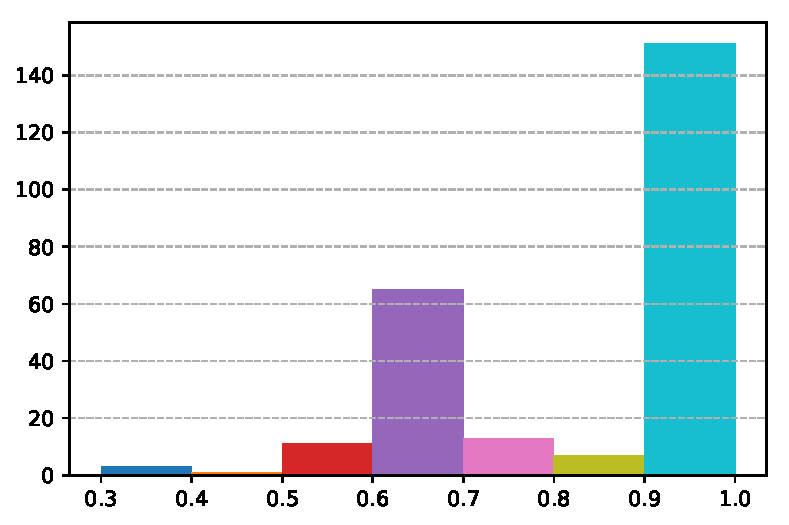
\includegraphics[width=0.5\textwidth]{images/prestudy/confidence.pdf}
\label{pre:dist}
  \captionof{figure}{Confidence Historgram}%
}
\parbox[b]{0.48\textwidth}{\null
\centering

\begin{tabular}{@{}ll@{}}
\toprule
Type & Value  \\ \midrule
Average Confidence & 0.86 \\
Standard Derivation & 0.17 \\
Lowest Confidence & 0.35\\
Highest Confidence & 1.00\\
25th percentile average & 0.67\\
50th percentile average & 1.00\\
\bottomrule
\label{pre:conf-table}
\end{tabular}
    \captionof{table}[t]{Confidence (details)}%
}
\end{figure}

From the 251 sentences, 15 got a confidence below 0.6, four below 0.5. The most diffcult sentence is with a confidence of 0.35 for the class \emph{WORSE} was
\begin{quote}
Google shouldn't have mandated an inferior map app on the iphone:[OBJECT\_A] (as opposed to android:[OBJECT\_B]).
\end{quote}

It was labelled as \emph{BETTER} (0.72 trust), \emph{WORSE} (0.85 trust) and \emph{NO\_COMP} (0.82 trust). In my mind, the class \emph{WRONG} is correct here, as the object iphone is inferior to android on the aspect of \emph{map app}.

The following sentence was assigned to \emph{BETTER} (0.37 confidence), although it should belong to \emph{UNCLEAR}.
\begin{quote}
Not to mention that the iphone:[OBJECT\_A] and android:[OBJECT\_B] phones deliver a far superior user experience overall
\end{quote}
However, the annotator for \emph{UNCLEAR} only had 0.87 trust, while the one for \emph{BETTER} had 1 (third one was \emph{NO\_COMP} with 0.82 trust).\newline

All things considered, the result of the prestudy is satisfactory since the annotators agreed in the majority of decisions. 


%As a baseline, I annotated the sentences\footnote{See appendix} according to the guidelines discussed in section \ref{sec:annotation-guidelines}. The resulting label distribution is shown in figure \ref{fig:pre-class-dist}. Tu summarize, 21.8\% of the sentences are comparative; \texttt{BETTER} is the dominant class.

\subsection{Main Study}
